% Compact RadarConf 2027 figures.

\newcommand{\radarconfArchitecture}{%
\begin{figure}[t]
\centering
\resizebox{\columnwidth}{!}{%
\begin{tikzpicture}[font=\scriptsize,node distance=4mm and 4mm,
box/.style={draw,rounded corners,align=center,minimum height=6.5mm,minimum width=20mm,fill=black!3},
arr/.style={-Latex,thick}]
\node[box] (state) {Estimated\\PHY state};
\node[box, right=of state] (gate) {Physics\\gate};
\node[box, right=of gate] (rel) {Joint-QoS\\reliability};
\node[box, right=of rel] (sel) {Select\\or abstain};
\draw[arr] (state) -- (gate);
\draw[arr] (gate) -- node[above]{admissible} (rel);
\draw[arr] (rel) -- (sel);
\end{tikzpicture}}
\caption{Admissibility-first control. Physically unsupported PC-FMCW actions are removed before uncertainty-aware joint sensing/communication qualification.}
\label{fig:radarconf-architecture}
\end{figure}}

\newcommand{\radarconfMainResults}{%
\begin{figure*}[t]
\centering
\begin{minipage}{0.49\textwidth}
\centering
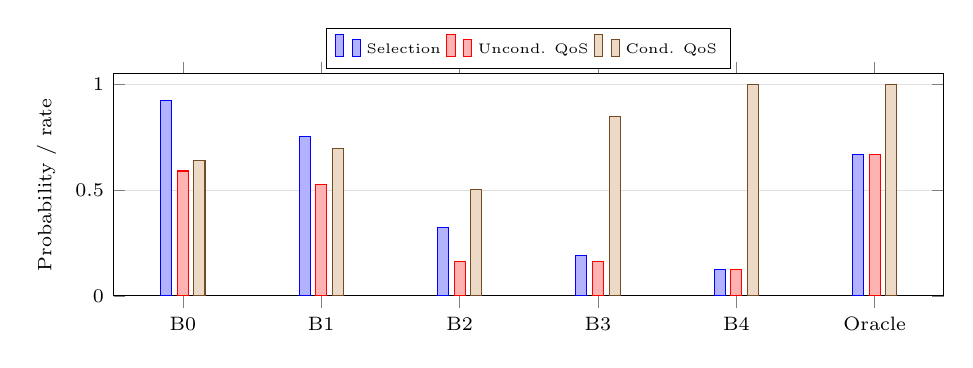
\begin{tikzpicture}
\begin{axis}[
width=\linewidth,height=4.4cm,
ybar,bar width=4pt,
ymin=0,ymax=1.05,
ylabel={Probability / rate},
symbolic x coords={B0,B1,B2,B3,B4,Oracle},xtick=data,
legend style={at={(0.5,1.02)},anchor=south,legend columns=3,font=\tiny},
tick label style={font=\scriptsize},label style={font=\scriptsize},
ymajorgrids=true,major grid style={black!12}]
\addplot coordinates {(B0,0.9235833)(B1,0.7531667)(B2,0.3225833)(B3,0.1906667)(B4,0.1223333)(Oracle,0.6666667)};
\addplot coordinates {(B0,0.5904167)(B1,0.5259167)(B2,0.16175)(B3,0.16175)(B4,0.1223333)(Oracle,0.6666667)};
\addplot coordinates {(B0,0.6392673)(B1,0.6982740)(B2,0.5014208)(B3,0.8483392)(B4,1.0)(Oracle,1.0)};
\legend{Selection,Uncond. QoS,Cond. QoS}
\end{axis}
\end{tikzpicture}
\end{minipage}\hfill
\begin{minipage}{0.49\textwidth}
\centering
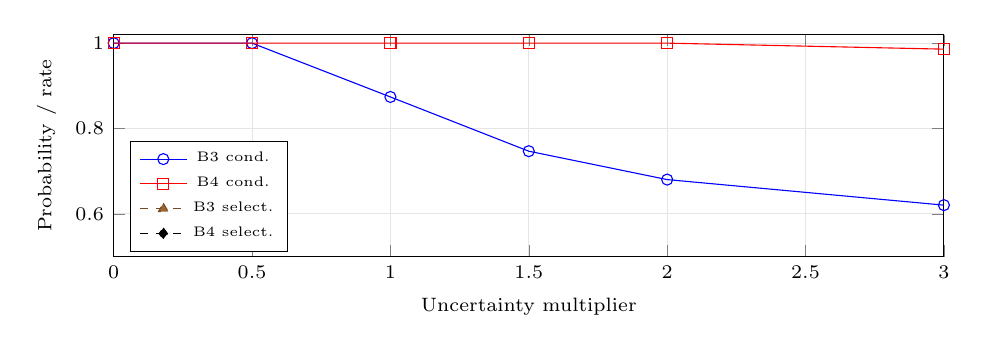
\begin{tikzpicture}
\begin{axis}[
width=\linewidth,height=4.4cm,
xlabel={Uncertainty multiplier},
ylabel={Probability / rate},
xmin=0,xmax=3,ymin=0.5,ymax=1.02,
legend style={font=\tiny,at={(0.02,0.02)},anchor=south west},
tick label style={font=\scriptsize},label style={font=\scriptsize},
grid=major,major grid style={black!10}]
\addplot+[mark=o] coordinates {(0,1)(0.5,1)(1,0.8739)(1.5,0.7468)(2,0.6803)(3,0.6204)};
\addplot+[mark=square] coordinates {(0,1)(0.5,1)(1,1)(1.5,1)(2,1)(3,0.9859)};
\addplot+[mark=triangle*,dashed] coordinates {(0,0.1667)(0.5,0.1667)(1,0.185)(1.5,0.1975)(2,0.2033)(3,0.2283)};
\addplot+[mark=diamond*,dashed] coordinates {(0,0.1667)(0.5,0.1617)(1,0.125)(1.5,0.1117)(2,0.0975)(3,0.0592)};
\legend{B3 cond.,B4 cond.,B3 select.,B4 select.}
\end{axis}
\end{tikzpicture}
\end{minipage}
\caption{Left: frozen paired benchmark over 12,000 state/seed units per policy. Right: increasing state uncertainty contracts B4's selected operating region while preserving higher conditional joint QoS until the strongest tested uncertainty setting.}
\label{fig:radarconf-results}
\end{figure*}}
